%
% Comment utiliser l'application ?
%
\newpage % nouvelle page
\section{Utilisation de {\nomApplication}/{\nomLogiciel}}

\subsection{Matériel nécessaire}
L'utilisation de l'application {\nomApplication} et du programme {\nomLogiciel} nécessite un matériel spécifique. Ce matériel a été défini avec le client et a été validé via tests. CANvengers ne garantit pas le bon fonctionnement du projet {\guillemetleft} {\projectName} {\guillemetright}. Le matériel testé est le suivant :
\begin{itemize}
    \item Banc de Test : KERAVAL Banc de Test ;
    \item Ordinateur : Linux Ubuntu (64-bit) ;
    \item Passerelle Raspberry-CAN : PEAK PCAN;USB IPEH-002021 175459 ;
    \item Passerelle Tableau de Bord-CAN : RS485/CAN HAT;
    \item Raspberry : pi 3B+ ;
    \item Smartphone : Samsung Galaxy A20e sous système Android 9.
\end{itemize}

\subsection{Logiciels nécessaires}
L'utilisation du système développé dans ce projet nécessite l'installation de certains logiciels :
\begin{itemize}
    \item Application {\nomApplication} : version 2.0.0 ;
    \item Programme {\nomLogiciel} : version 2.0.0 ;
    \item \hyperref[ICSim]{Simulateur ICSim} : version du 12/06/2020.
\end{itemize}
Pour installer ces logiciels veuillez suivre les instructions du \hyperref[INST]{Manuel\_Installation\_SANS\_B1\_2024}.\\

\subsection{Préparation}
En fonction de l'utilisation souhaitée, Utilisateur peut n'avoir besoin que d'une partie du matériel.

\subsubsection{Application {\nomApplication} seule}
Pour une utilisation de l'application {\nomApplication} seule, les éléments suivants sont nécessaires :
\begin{itemize}
    \item Application {\nomApplication} ;
    \item Smartphone.
\end{itemize}

\subsubsection{Utilisation de la Raspberry Pi}
Pour une utilisation de l'application {\nomApplication} avec la Raspberry Pi, les éléments suivant sont nécessaires :
\begin{itemize}
    \item Application {\nomApplication} ;
    \item Programme {\nomLogiciel} ;
    \item Raspberry ;
    \item Smartphone.
\end{itemize}

\subsubsection{Utilisation du Simulateur ICSim}
Pour une utilisation de l'application {\nomApplication} avec la Raspberry Pi et le Simulateur ICSim, les éléments suivant sont nécessaires :
\begin{itemize}
    \item Application {\nomApplication} ;
    \item Ordinateur ;
    \item Passerelle Raspberry-CAN ;
    \item Passerelle Tableau de Bord-CAN ;
    \item Programme {\nomLogiciel} ;
    \item Raspberry ;
    \item Simulateur ICSim ;
    \item Smartphone.
\end{itemize}

\subsubsection{Utilisation du Banc de Test}
Pour une utilisation de l'application {\nomApplication} avec la Raspberry Pi, les éléments suivant sont nécessaires :
\begin{itemize}
    \item Application {\nomApplication} ;
    \item Banc de Test ;
    \item Passerelle Tableau de Bord-CAN ;
    \item Programme {\nomLogiciel} ;
    \item Raspberry Pi ;
    \item Smartphone.
\end{itemize}

\subsubsection{Utilisation du Simulateur ICSim et du Banc de Test}
Pour une utilisation de l'application {\nomApplication} avec la Raspberry Pi, les éléments suivant sont nécessaires :
\begin{itemize}
    \item Application {\nomApplication} ;
    \item Banc de Test ;
    \item Ordinateur ;
    \item Passerelle Raspberry-CAN ;
    \item Passerelle Tableau de Bord-CAN ;
    \item Programme {\nomLogiciel} ;
    \item Raspberry Pi ;
    \item Simulateur ICSim ;
    \item Smartphone.
\end{itemize}

\subsubsection{Tests}
Pour l'exécution des tests, les logiciels suivants sont nécessaires :
\begin{itemize}
    \item Tests du programme {\nomLogiciel} :
    \begin{itemize}
        \item GNU Compiler Collection : Logiciel utilisé pour compiler les tests ;
        \item CMocka : Module de tests (notamment utilisé pour les tests unitaires) ;
        \item Apache JMeter : Logiciel utilisé pour les tests de serveurs.
    \end{itemize}
    \item Tests de l'application {\nomApplication} :
    \begin{itemize}
        \item JUnit : Logiciel utilisé pour les tests unitaires ;
        \item Robot Framework : Logiciel utilisé pour les tests de validation.
    \end{itemize}
\end{itemize}

\subsection{Branchement}
Pour l'utilisation du matériel veuillez suivre le branchement décrit ci-dessous selon votre utilisation.

\subsubsection{Simulateur ICSim}

Pour utiliser le Simulateur ICSim avec notre système, il faut pouvoir connecter votre PC avec la Raspberry Pi. Pour cela, vous pouvez utiliser le PCAN-USB de PEAK. Connectez la partie USB à votre PC et la partie CAN à la Raspberry Pi.\\

Voici le lien du site de PCAN-USB : \href{https://www.peak-system.com/PCAN-USB.199.0.html?&L=2}{Interface CAN pour USB}.\\

Il y a 3 pins importantes sur les 9 pins du connecteur CAN :
\begin{itemize}
    \item CAN\_L : pin 2 ;
    \item CAN\_H : pin 7 ;
    \item GND : pin 6.
\end{itemize}

\begin{minipage}
    \textwidth
    \centering
    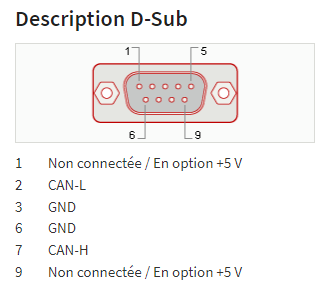
\includegraphics[width=0.5\textwidth]{../figures/D-Sub_PEAK.png}
    \captionof{figure}{Description des pins du PCAN-USB}
\end{minipage}

Pour connecter ses pins à la Raspberry Pi, vous pouvez utiliser un connecteur connecteur DB9 femelle et souder des fils sur les pins 2, 7 et 6.\\

Connectez ensuite les fils CAN\_H et CAN\_L aux pins du RS485 CAN HAT et GND à une pin GND de la Raspberry Pi.\\

Attention, pour utiliser ICSim, il vous faut utiliser un RS485 CAN HAT dont la résistance de terminaison est soudée.\\

\subsubsection{Banc de Test}

Pour utiliser le Banc de Test, vous n'avez pas besoin d'un connecteur DB9 supplémentaire, celui-ci est déjà présent sur le Banc de Test.\\

Trouvez le connecteur DB9 dans le Banc de Test, de la même manière que pour le connecteur DB9 précédent, les pins 2 et 7 sont soudées à des fils que vous pouvez directement connecter au RS485 CAN HAT.\\

Attention cependant, pour utiliser le Banc de Test, il vous faut utiliser un RS485 CAN HAT dont la résistance de terminaison est désoudée.\\

\subsubsection{Banc de Test et Simulateur ICSim}

Pour utiliser à la fois le Banc de Test et le simulateur ICSim, il vous suffit de connecter le connecteur DB9 du Banc de Test au PCAN-USB que vous reliez à votre PC. Reliez également les pins 2 et 7 du Banc de Test au RS485 CAN HAT.\\

De la même manière que pour les deux autres utilisations, vous devez utiliser un RS485 CAN HAT dont la résistance de terminaison est désoudée.\\

\subsection{Démarrage}

Afin que le système fonctionne au mieux, nous vous proposons de suivre les étapes suivantes dans l'ordre indiqué.

\subsubsection{Banc de Test}

Dans le cadre de notre projet, nous tenons à préciser que nous n'avons pas utilisé le Banc de Test, mais uniquement le simulateur ICSim. Par conséquent, nous ne disposons pas des informations nécessaires pour décrire en détail le cycle d'allumage du dispositif. Notre travail s'est principalement concentré sur l'utilisation du simulateur et la mise en œuvre des fonctionnalités requises.

\subsubsection{Simulateur ICSim}

Si vous souhaitez utiliser le Simulateur ICSim, commencez pas brancher le PCAN-USB à votre PC et à la Raspberry Pi.\\
Si vous le branchez sur un OS Linux, vous n'avez rien à faire, le driver permettant d'utiliser le PCAN-USB est déjà installé sur le noyau Linux.\\
Sinon, vous avez besoin de télécharger le driver sur le site de PEAK : \href{https://www.peak-system.com/PCAN-USB.199.0.html?&L=2}{Support PEAK}.\\
Si le PCAN-USB est branché et que le driver est installé, la LED rouge du PCAN-USB doit être allumée.\\

Commencez par activer le CAN sur votre ordinateur : 
\begin{itemize}
    \item Dans un terminal, tapez :
\vspace{-1.8\baselineskip} 
\begin{lstlisting}
    sudo ip link set can0 down
    sudo ip link set can0 type can bitrate 125000
    sudo ip link set can0 up
\end{lstlisting}
    \item Vérifiez que le CAN est bien activé :
\vspace{-1.8\baselineskip} 
\begin{lstlisting}
    sudo ip -details link show can0
\end{lstlisting}
Vous devriez voir ceci : 
\vspace{-1.8\baselineskip}
\begin{lstlisting}
    3: can0: <NOARP,UP,LOWER_UP,ECHO> mtu 16 qdisc pfifo_fast state UP mode DEFAULT group default qlen 10
    link/can  promiscuity 0 minmtu 0 maxmtu 0 
    can state ERROR-ACTIVE (berr-counter tx 0 rx 95) restart-ms 0 
	  bitrate 125000 sample-point 0.875 
	  tq 500 prop-seg 6 phase-seg1 7 phase-seg2 2 sjw 1
	  pcan_usb: tseg1 1..16 tseg2 1..8 sjw 1..4 brp 1..64 brp-inc 1
	  clock 8000000 numtxqueues 1 numrxqueues 1 gso_max_size 65536 gso_max_segs 65535 parentbus usb parentdev 2-2.1:1.0 
\end{lstlisting}
\end{itemize}

Pour rappel, le bus CAN est fonctionnel quand il est dans l'état ERROR-ACTIVE. Dans l'état STOPPED, il n'a pas démarré. Dans l'état ERROR-PASSIVE, il est en erreur et il faut le redémarrer pour qu'il fonctionne à nouveau.\\

Lorsque le bus CAN est fonctionnel, la LED rouge du PCAN-USB clignote lentement (elle cligonte rapidement lorsque des trames sont émises).\\

Dès que le bus CAN est fonctionnel, vous pouvez lancer le Simulateur ICSim :
\begin{enumerate}
    \item Ouvrez un terminal et placez vous dans le dossier ICSim ;
    \item Tapez :
\vspace{-1.8\baselineskip}
\begin{lstlisting}
    ./icsim can0
\end{lstlisting}
    \item Ouvrez un second terminal et placez vous dans le dossier ICSim ;
    \item Tapez :
\vspace{-1.8\baselineskip}
\begin{lstlisting}
    ./controls can0
\end{lstlisting}
\end{enumerate}

Cela est sensé vous ouvrir deux fenêtres, une pour le Simulateur ICSim et une pour le contrôleur : 

\begin{minipage}
    \textwidth
    \centering
    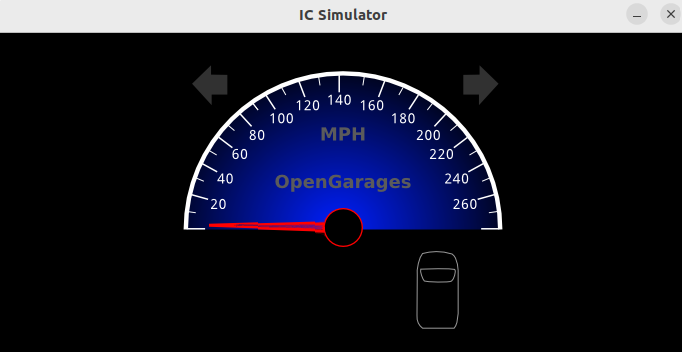
\includegraphics[width=0.80\textwidth]{../figures/ICSIM.png}
    \captionof{figure}{ICSim}
    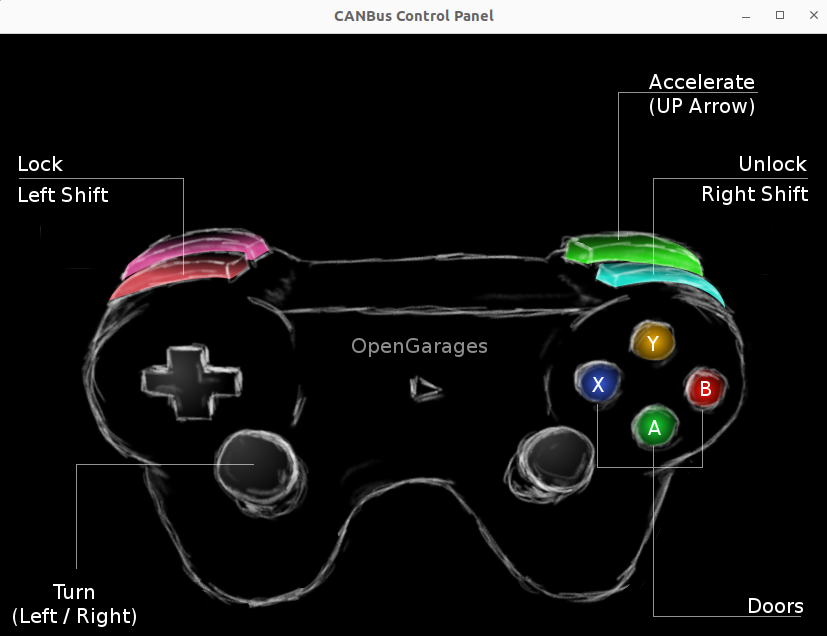
\includegraphics[width=\textwidth]{../figures/CONTROLEUR.png}
    \captionof{figure}{Contrôleur}
\end{minipage}

le Simulateur ICSim est démarré, vous pouvez voir toutes les trames émises entre le simulateur et le contrôleur grâce aux commandes suivantes :
\begin{itemize}
    \item Permet d'afficher toutes les trames sniffées :
\vspace{-1.8\baselineskip}
\begin{lstlisting}
    candump can0
\end{lstlisting}
    \item Permet de n'afficher que les nouvelles trames sniffées (évite d'afficher les même trames à répétition) :
\vspace{-1.8\baselineskip}
\begin{lstlisting}
    cansniffer -c can0
\end{lstlisting}
\end{itemize}

\subsubsection{Programme {\nomLogiciel}}

Pour utiliser le programme {\nomLogiciel}, commencez par vous connecter à la Raspberry Pi via SSH, ou, si vous préférez, connectez un écran et un clavier à la Raspberry Pi.\\

Ouvrez un terminal de la Raspberry Pi et placez vous dans le dossier /home/pi. \\

Vérifiez que le programme {\nomLogiciel} est bien présent dans le dossier, sinon, veuillez lire le \hyperref[INST]{Manuel\_Installation\_SANS\_B1\_2024}, dans la section "Installation du programme {\nomLogiciel}".\\

Pour lancer le programme {\nomLogiciel}, tapez :
\vspace{-1.8\baselineskip}
\begin{lstlisting}
    sudo ./CANgateway.out
\end{lstlisting}
(Entrez le mot de passe si nécessaire)\\

Lorsque le programme est lancé, vous pouvez voir le message suivant s'afficher dans la console :
\vspace{-2.5\baselineskip}
\begin{lstlisting}
    Lancement du programme
\end{lstlisting}

\subsubsection{Application {\nomApplication}}
Si l'application {\nomApplication} est installée sur le Smartphone, cliquer sur l'icone de l'application {\nomApplication} sur l'écran.

Si l'application {\nomApplication} n'est pas installée sur le Smartphone, suivre le \hyperref[INST]{Manuel\_Installation\_SANS\_B1\_2024}.

\subsection{Manipulation}
Lors de votre utilisation du projet, seuls les fonctionnalités décrites dans \hyperref[SPEC]{dossier\_de\_specifi-cation\_SPEC\_B1\_2024} et \hyperref[plan_de_test]{plan\_de\_test \_TEST\_B1\_2024}. Toute utilisation de l'application {\nomApplication} et du programme {\nomLogiciel} sortant de ce cadre peut amener à des disfonctionnements dont l'équipe {\teamName} n'est pas responsable.

\subsubsection{Application {\nomApplication}}
Durant l'utilisation normale du projet, plusieurs interactions entre Utilisateur et l'application {\nomApplication} sont prévues. Ces interactions sont les suivantes :

\begin{itemize}
    \item Partie haute de l'écran
    \begin{itemize}
        \item Ajout de trame
        \item Ajout d'objet
        \item Défilement
        \item Déroulement des menu d'objet
        \item Mise en marche/arrêt de l'envoi de trames
        \item Reconnexion
        \item Séléctions d'éléments
        \item Suppression d'éléments
    \end{itemize}
    \item Partie basse de l'écran
    \begin{itemize}
        \item Défilement
        \item Enregistrement du sniffer
        \item Mise en marche/arrêt du sniffer
        \item Nettoyage du sniffer
    \end{itemize}
\end{itemize}

L'écran de l'application {\nomApplication} présente une partie d'interaction avec le Simulateur ICSim et une partie sniffer CAN.

\paragraph{Partie interaction avec le simulateur}
\medskip
La partie {\guillemetleft} haute {\guillemetright} (interaction avec le smiffer) permet d'intéragir avec le Simulateur ICSim. On y observe l'état de la connexion au programme {\nomLogiciel}. On peut ajouter ou supprimer des objets, et dans ces mêmes objets, ajouter ou supprimer des trames. Enfin, on peut y ordonner l'envoi de trames. Pour une explication détaillée de son fonctionnement, veuillez vous réferez au \hyperref[SPEC]{dossier\_de\_specification\_SPEC\_B1\_2024}.

\paragraph{Partie basse de l'écran}
La partie sniffer (partie basse de l'écran) présente les trames CAN envoyées et reçues par la Raspberry Pi lorsqu'il y en a. Lorsque la Raspberry Pi n'est pas encore connectée, un commentaire indique qu'il n'y a pas de trames actuellement. Pour une explication détaillée de son fonctionnement, veuillez vous réferez au \hyperref[SPEC]{dossier\_de\_specification\_SPEC\_B1\_2024}.

\subsubsection{Programme {\nomLogiciel}}
Durant l'utilisation normale du projet, aucune interaction entre Utilisateur et le programme {\nomLogiciel} n'est prévue.

\subsubsection{Simulateur ICSim}
Durant l'utilisation normale du projet, Utilisateur peut être amené à interagir avec le Simulateur ICSim. Ces interactions seront l'activation d'actionneurs et la lecture des informations affichées par le Tableau de Bord.
\newline
Pour plus d'informations concernant la manipulation du Simulateur ICSim, voir document README.md disponible sur la {\href{https://github.com/zombieCraig/ICSim}{page github du projet}}.


\subsubsection{Programme {\nomLogiciel}}
Durant l'utilisation normale du projet, il vous est possible de voir les potentiels messages d'erreurs dans la console. \\
Vous pouvez arrêter le programme {\nomLogiciel} en appuyant sur la touche "Ctrl + C" dans la console. Cela affichera le message suivant :
\vspace{-1.8\baselineskip}
\begin{lstlisting}
    SIGINT intercepté : demande d`arrêt du programme
    Arrêt du programme
\end{lstlisting}

Le programme {\nomLogiciel} s'arrête alors.

Si le programme ne s'arrête pas, il se peut que le client TCP soit encore connecté, veillez à bien fermer l'application {\nomApplication} avant de fermer le programme {\nomLogiciel} afin de forcer la déconnexion du client TCP.

\subsubsection{Simulateur ICSim}
Durant l'utilisation normale du projet, Utilisateur peut être amené à interagir avec le Simulateur ICSim. Ces interactions seront l'activation d'actionneurs et la lecture des informations affichées par le Tableau de Bord.
\newline
Pour plus d'informations concernant la manipulation du Simulateur ICSim, voir document README.md disponible sur la {\href{https://github.com/zombieCraig/ICSim}{page github du projet}}.

\subsubsection{Banc de Test}
Durant l'utilisation normale du projet, Utilisateur peut être amené à interagir avec le Banc de Test. Ces interactions seront l'activation d'actionneurs et la lecture des informations affichées sur le Tableau de Bord.

\subsection{Tests}
Lors de l'exécution des codes de test, certaines étapes sont à respecter.

\subsubsection{JMeter}

Pour exécuter les tests du serveur TCP du Postman dans JMeter, il faut tout d'abord lancer le programme {\nomLogiciel}. Pour lancer le programme {\nomLogiciel}, tapez :
\vspace{-1.8\baselineskip}
\begin{lstlisting}
    sudo ./CANgateway.out
\end{lstlisting}
(Entrez le mot de passe si nécessaire)\\
Il faut ensuite lancer JMeter. Pour ce faire, accédez au dépôt C du projet, et allez dans le répertoire \path{Git/c/production/jmeter_test/}. Si ce n'est pas déjà fait, veuillez modifier le Makefile et modifier le chemin absolu vers JMeter, de façon à ce qu'il corresponde à votre installation.\\
Ensuite pour compiler et lancer JMeter, exécutez les commandes suivantes :
\vspace{-1.8\baselineskip}
\begin{lstlisting}
    make all
\end{lstlisting}
\vspace{-1.8\baselineskip}
\begin{lstlisting}
    ./customLaunch.sh
\end{lstlisting}
Enfin, une fois JMeter lancé, appuyez sur la flèche verte pour démarrez le test. 

\subsubsection{Robot Framework}

% A faire : Description execution Robot Framework

\subsubsection{Tests unitaires CMocka}

Vous pouvez effectuer des tests unitaires d'encodage et de décodage de chaînes de caractères en utilisant le programme {\nomLogiciel}.\\

Ces tests sont exécutables sur cible Raspberry Pi mais également sur PC.\\

Selon votre choix, la compilation du programme de tests de {\nomLogiciel} sera différente, veuillez vous référer au [Guide d'installation] pour la compilation.\\

Quelque soit la cible, les tests sont exécutables de la même manière.\\

Ouvrez un terminal de la Raspberry Pi ou du PC et placez vous dans le dossier contenant l'exécutable de tests, tapez :
\vspace{-1.8\baselineskip}
\begin{lstlisting}
    ./CANgateway_test.out
\end{lstlisting}

Trois tests sont alors exécutés, vous pouvez voir leur résultats dans la console.\\
